% Confronto com a literatura recente (nove artigos), o patamar inferior do FS e benchmarks
%======================================================================
\section{Confronto com a literatura recente}\label{sec:literatura}
%======================================================================

Nove trabalhos posteriores ao de Rahardjo et al.\ (2007) foram lidos integralmente e confrontados com os resultados
das Se\c{c}\~oes~\ref{sec:rahardjo} e \ref{sec:contraexemplos}: Ali et al.\ (2014), Zhang et al.\ (2014),
Dou et al.\ (2015), Tang et al.\ (2018), Wang, Vardon e Hicks (2018), Ran et al.\ (2018), Liu e Wang (2021),
Wang, Idinger e Wu (2021) e Pradhan et al.\ (2022). A Tabela~\ref{tab:literatura} resume as hip\'oteses de cada um.

\begin{table}[h!]
\centering\small
\caption{Hip\'oteses dos trabalhos analisados. $\psi$: \^angulo de dilat\^ancia; a \'ultima coluna d\'a
$\tan\phi'/\tan\alpha$ e $c'$ (o FS de talude infinito sem suc\c{c}\~ao \'e $\tan\phi'/\tan\alpha$ com $c'=0$).}
\label{tab:literatura}
\begin{tabular}{p{2.5cm}p{3.6cm}p{1.2cm}p{1.5cm}p{1.6cm}p{2.4cm}}
\toprule
Trabalho & Modelo & $\chi$ & $\psi$ & ar & $\tan\phi'/\tan\alpha$; $c'$\\
\midrule
Rahardjo 2007 & SEEP/W + equil\'ibrio-limite & 1 & -- & $p_a=0$ & 0,49; 10~kPa\\
Ali 2014 & coluna 1D (HYDRUS) + talude infinito & $S_e$ & -- & $p_a=0$ & 0,96; 0\\
Zhang 2014 & est\'atico, GLE & 6 leis & -- & $p_a=0$ & 0,57; 10~kPa\\
Dou 2015 & coluna 1D (FLAC) + talude infinito & $S_e$ & -- & ``ignorado'' & 0,75; 5~kPa\\
Tang 2018 & SEEP/W + SLOPE/W & 0,639 & -- & $p_a=0$ & 0,49; 0\\
Wang, Vardon e Hicks 2018 & MPM acoplado & $S$ & 0,1$^\circ$ & $p_a=0$ & 1,0; 20$\to$0,1~kPa\\
Ran 2018 & Richards 3D + talude infinito & 1 & -- & $p_a=0$ & 0,82; $\approx1$~kPa\\
Liu e Wang 2021 & Abaqus acoplado + MPM & $S_w$ & 0 & $p_a=0$ & 0,81; 0\\
Wang 2021 & centr\'ifuga (30~$g$) & ($\approx1$) & contr\'atil & n\~ao medido & 0,62; 0\\
Pradhan 2022 & PLAXIS acoplado & $S_e$ & n\~ao inf. & $p_a=0$ & corte 0,25; 3~kPa\\
\bottomrule
\end{tabular}
\end{table}

As aparentes contradi\c{c}\~oes entre esses trabalhos, e deles com Rahardjo et al., organizam-se em seis teses.

\subsection{T0. Os trabalhos est\~ao em regimes diferentes}

Pelo menos seis dos nove analisam taludes que s\'o ficam de p\'e pela suc\c{c}\~ao ($c'\approx0$ e
$\tan\phi'/\tan\alpha<1$). Nesse regime a margem at\'e a ruptura \'e de 0,2--3~kPa (Ali, Ran, Wang 2021), menor do que
os efeitos tratados como de segunda ordem: a press\~ao do ar aprisionado (36--38~kPa no item A2), a suc\c{c}\~ao gerada
pela dilat\^ancia e a troca da lei de $\chi$ (FS inicial de 1,28 para 1,63 na coluna de Ali). Rahardjo et al., com
$c'=10$~kPa, est\~ao em outro regime; por isso suas conclus\~oes (geometria e NA secund\'arios, patamar de FS) n\~ao se
transferem.

\subsection{T1. A dilat\^ancia decide se o modelo acoplado prev\^e ruptura}

Os modelos acoplados que rompem usam $\psi\approx0$ (Liu e Wang; Wang, Vardon e Hicks; provavelmente Pradhan, pelo
padr\~ao do PLAXIS) e o solo dos ensaios de Wang et al.\ (2021) \'e contr\'atil. Nenhum dos nove varia $\psi$. No
NeoPZ (item A1), com $I_r\ge36$~mm/h o modelo acoplado com $\psi=\phi'/2$ ou $\psi=\phi'$ para em FS 1,00--1,01 sem
romper; com $\psi=0$ o transiente perde o equil\'ibrio entre 11,75 e 15,5~h e o FS desce a 0,96. A dilat\^ancia decide
se h\'a ruptura, mas explica pouco do valor do patamar: sem ela o patamar desce s\'o de 1,00 a 0,96, contra 0,84--0,85
no modelo desacoplado.

\subsection{T2. As leis de dura\c{c}\~ao e de padr\~ao de chuva reduzem-se ao volume infiltrado}

Ran (limiar de $\approx150$~mm acumulados de 7,5 a 80~mm/h), Tang (ruptura com 59--71~mm em todas as dura\c{c}\~oes e
nos padr\~oes t\'ipicos), Ali ($t_f\approx$ d\'eficit de armazenamento/fluxo) e Dou e Pradhan (leis de dura\c{c}\~ao com
$u_w=0$ na superf\'icie ou $I/k_s\approx2$--5) s\~ao casos da mesma regra: o que governa \'e o volume infiltrado,
limitado por $k_s$. Tang acrescenta o centr\'oide temporal da chuva ($\pm0{,}1$ no FS com o mesmo volume). O item A6
restringe a regra: no $f_{10}$ os mesmos 60,5~m$^3$/m infiltram em todas as dura\c{c}\~oes e o FS m\'inimo vai de 1,31
(3~h) a 1,78 (72~h); com volume fixo, o pior caso testado \'e a chuva com $I_r$ mais pr\'oximo de $k_s$, compat\'ivel
com $t^*\approx V/k_s$ (Eq.~\eqref{eq:tcrit}). E no item A2, com ar ativo, menos \'agua d\'a FS menor.

\subsection{T3. O patamar inferior \'e do problema de contorno}

A profundidade da ruptura ``profunda'' de Ali \'e a da rocha; Dou chega a FS $=0{,}27$ com rocha a 3~m e coluna 1D; Ran
tem um segundo patamar quando a caixa fechada satura; para Zhang o piso \'e o FS com $\phi^b=0$ e o teto, o mecanismo
profundo que busca o NA; no item A3 o patamar vai de 0,63 a 1,05 s\'o pela orienta\c{c}\~ao do tensor. A
Se\c{c}\~ao~\ref{sec:patamar} mostra que o patamar \'e o FS do talude saturado at\'e a superf\'icie.

\subsection{T4. A lei de $\chi$ \'e de primeira ordem}

Cinco leis em nove trabalhos ($\chi=1$, $S_e$, $S_w$, constante, n\~ao lineares). Em Zhang et al.\ o mesmo talude vai de
FS 0,90 a 1,92 conforme a lei. A press\~ao de entrada de ar dos solos de Rahardjo (Fredlund--Xing com
$n=m=1$) \'e $\approx2{,}7$, 13 e 27~kPa para $a=10$, 50 e 100~kPa; pelo crit\'erio de Zhang ($\phi^b=\phi'$ s\'o com
AEV $>200$~kPa) a hip\'otese $\chi=1$ n\~ao se justifica em nenhum dos tr\^es solos. O efeito concentra-se no FS
inicial e no tempo at\'e a ruptura; na ruptura ($S\to1$) \'e pequeno (Ali $\approx4\%$, Ran $\le0{,}02$).

\subsection{T5. Ar: os modelos usam $p_a=0$, quase sempre em dom\'inios fechados ao ar}

Os modelos num\'ericos usam $p_a=0$ (o ensaio de Wang 2021 n\~ao mede $p_a$). Rocha na base (Ali, Dou), base e
laterais imperme\'aveis (Liu, Ran, Wang e Hicks), base imperme\'avel e laterais sem fluxo acima do NA (Tang, com carga
imposta abaixo dele), caixa fechada (Wang 2021) e solo pouco perme\'avel com NA profundo (Pradhan): em todos, o ar s\'o
sai pela superf\'icie. Em Ran, a lei de Boyle sem escape d\'a um limite superior de 50--190~kPa para a press\~ao do ar,
contra uma margem de 2,5~kPa; em Tang, a sensibilidade $\mathrm{d}\,\mathrm{FS}/\mathrm{d}V\approx-0{,}004$/mm faz o
efeito do item A2 ($-0{,}08$ a $-0{,}22$) equivaler a 20--55~mm a mais de chuva (com a sensibilidade do NeoPZ para os
mesmos dados, $\approx-0{,}0016$/mm, a 2,5 vezes isso; Tabela~\ref{tab:tang}).

\subsection{Nota de m\'etodo e inconsist\^encias encontradas}

Com $c'=0$, a redu\c{c}\~ao de resist\^encia por elementos finitos tende a encontrar rupturas superficiais na face assim
que ela umedece (talude infinito sem suc\c{c}\~ao: FS $=0{,}49$ em Tang); o equil\'ibrio-limite as evita por
restri\c{c}\~oes de busca. Pradhan et al.\ adotam $c'=3$~kPa exatamente por isso.

Inconsist\^encias internas: Ali (a conclus\~ao sobre o comprimento de correla\c{c}\~ao contradiz as Figs.~8 e 17; a
Eq.~7 conta $1/\cos\alpha$ duas vezes); Zhang (limiar de 10 e de 20~kPa usados como o mesmo); Dou (par\^ametros de van
Genuchten incompat\'iveis com a Fig.~3); Tang (a mesma distribui\c{c}\~ao GEV nas tr\^es dura\c{c}\~oes); Wang, Vardon e
Hicks (a permeabilidade do ensaio de Liakopoulos n\~ao reproduz a Fig.~3; a frente avan\c{c}a 4 vezes mais devagar que
o $k$ declarado); Ran ($c'$ em Pa na tabela, mas as figuras s\'o fecham com kPa); Liu e Wang ($\phi'=30^\circ$ na tabela e
$33^\circ$ no texto); Wang 2021 (o limiar $I$--$D$ n\~ao separa ruptura de n\~ao ruptura); Pradhan (FS $<1$ em junho,
quando a ruptura foi em julho, e rein\'icio da simula\c{c}\~ao em 1$^\circ$ de julho).

%======================================================================
\section{Benchmarks com a literatura}\label{sec:benchmarks}
%======================================================================

As op\c{c}\~oes acrescentadas ao programa (\texttt{SlopeRainfall}) para estes casos: resist\^encia, peso,
elasticidade, condutividade e porosidade por camada; $\chi$ constante (s\'o na suc\c{c}\~ao, isto \'e,
$\tan\phi^b=\chi\tan\phi'$ e $\chi=1$ com $p_w>p_a$), $\chi=S_w$ ou $\chi=S_e$; curvas de Fredlund--Xing ou van
Genuchten--Mualem; malhas poligonais com camadas paralelas \`a superf\'icie (\texttt{scripts/malha\_poligono.py}); NA
poligonal; hietogramas lidos de arquivo e padr\~oes lineares; evapora\c{c}\~ao limitada por uma suc\c{c}\~ao m\'axima;
infiltra\c{c}\~ao permanente como estado inicial; superf\'icie alagada ($I\to\infty$). Sem essas op\c{c}\~oes os
resultados anteriores se repetem exatamente.

\subsection{Zhang et al.\ (2014): leis de resist\^encia, casos est\'aticos}

Caso A: talude de 50$^\circ$ e 30~m ($\gamma=18$~kN/m$^3$, $c'=10$~kPa, $\phi'=34^\circ$), NA profundo e poligonal;
caso B: 30$^\circ$ e 20~m ($\phi'=24^\circ$), NA raso. Poro-press\~ao hidrost\'atica sem limite de suc\c{c}\~ao; FS por
redu\c{c}\~ao de resist\^encia no NeoPZ e GLE (Morgenstern--Price) no artigo.

\begin{table}[h!]
\centering\small
\caption{Zhang et al.\ (2014), Tabelas 4 e 5: FS m\'inimo do artigo e do NeoPZ.}\label{tab:zhang}
\begin{tabular}{llccc}
\toprule
caso & lei & artigo & NeoPZ & diferen\c{c}a\\
\midrule
A & $\phi^b=0$ ($\chi=0$) & 0,898 & 0,906 & $+0{,}9\%$\\
A & $\phi^b=15^\circ$ ($\chi=0{,}397$) & 1,414 & 1,444 & $+2{,}1\%$\\
A & $\phi^b=\phi'$ ($\chi=1$) & 1,920 & 1,919 & $-0{,}1\%$\\
A & Fredlund 1996, $\kappa=1$, SWCC1 ($\chi=S_w$) & 1,032 & 1,088 & $+5{,}4\%$\\
B & $\phi^b=0$ & 1,086 & 1,044 & $-3{,}9\%$\\
B & $\phi^b=15^\circ$ ($\chi=0{,}602$) & 1,133 & 1,100 & $-2{,}9\%$\\
B & $\phi^b=\phi'$ & 1,159 & 1,125 & $-2{,}9\%$\\
\midrule
A & $\chi=1$ com a suc\c{c}\~ao limitada a 75~kPa & -- & 1,656 & \\
\bottomrule
\end{tabular}
\end{table}

O acordo \'e de 0--5\%; no caso de $\chi=S_w$ a diferen\c{c}a vem da curva de Fredlund--Xing sem o fator de corre\c{c}\~ao
$C(\psi)$ no NeoPZ (o artigo usa $\psi_r=10$~kPa), que d\'a $S_w$ maior nas suc\c{c}\~oes altas. O \'ultimo caso
mostra o peso do limite de 75~kPa de Rahardjo et al.\ num talude com NA profundo: o FS cai de 1,92 para 1,66
($-14\%$), o mesmo efeito encontrado no item A4.

\subsection{Tang et al.\ (2018): intensidade, dura\c{c}\~ao e padr\~ao da chuva}

Talude de Rahardjo et al.\ (10~m, 45$^\circ$, NA 5~m abaixo do p\'e e inclinado a 7$^\circ$) com o solo da Tabela~1 do
artigo: $\gamma=20$~kN/m$^3$, $c'=0$, $\phi'=26^\circ$, $\phi^b=17{,}3^\circ$ ($\chi=0{,}6387$ na suc\c{c}\~ao),
$\theta_s=0{,}45$, $k_s=2\times10^{-6}$~m/s, Fredlund--Xing com $a=100$~kPa e $n=m=1$ e $k_w=k_s\Theta^4$ (a curva de
permeabilidade coincide com a Fig.~6 do artigo); suc\c{c}\~ao inicial limitada a 50~kPa; percola\c{c}\~ao
desacoplada com $p_a=0$ (SEEP/W no artigo); FS por redu\c{c}\~ao de resist\^encia nos instantes da grade de tempo do
artigo (SLOPE/W no artigo). Chuvas uniformes de 25,6 e 6,4~h e os padr\~oes lineares adiantado, uniforme e atrasado
com a mesma m\'edia (Tabela~\ref{tab:tang}, Fig.~\ref{fig:tang}).

\begin{table}[h!]
\centering\small
\caption{Tang et al.\ (2018): FS m\'inimo no NeoPZ (SRM) e queda por mm de chuva, medida contra o c\'alculo sem chuva
no mesmo instante; no artigo (Figs.~9 e 10, leitura), o FS inicial e a intensidade m\'edia $I_c$ (mm/h) em que o FS
m\'inimo chega a 1,0. $V$: volume de chuva. Sem chuva, o FS do NeoPZ \'e 1,331 no in\'icio e 1,324 em 4~h (o
m\'inimo).}\label{tab:tang}
\setlength{\tabcolsep}{3.5pt}
\begin{tabular}{lccccl}
\toprule
chuva & $I$ (mm/h) & $V$ (mm) & FS m\'inimo NeoPZ & queda por mm & artigo\\
\midrule
sem chuva & -- & 0 & 1,324 & -- & FS inicial 1,20\\
25,6~h, uniforme & 2,0 & 51 & 1,272 & 0,0016 & \\
 & 2,4 & 61 & 1,259 & 0,0015 & \\
 & 2,7 & 69 & 1,246 & 0,0016 & FS $=1$ com $I_c=2{,}70$\\
 & 3,0 & 77 & 1,234 & 0,0016 & \\
 & 3,5 & 90 & 1,208 & 0,0016 & \\
6,4~h, uniforme & 8 & 51 & 1,224 & 0,0020 & \\
 & 10 & 64 & 1,203 & 0,0019 & FS $=1$ com $I_c=9{,}7$\\
 & 12 & 77 & 1,173 & 0,0020 & \\
25,6~h, adiantado & 2,64 & 68 & 1,240 (em 16~h) & 0,0015 & $I_c=2{,}77$\\
25,6~h, uniforme & 2,64 & 68 & 1,246 & 0,0016 & $I_c=2{,}70$\\
25,6~h, atrasado & 2,64 & 68 & 1,240 & 0,0017 & $I_c=2{,}55$\\
\midrule
25,6~h, \texttt{fluxonormal=1} & 2,7 & 69 & 1,215 & 0,0020 & \\
\bottomrule
\end{tabular}
\end{table}

\begin{figure}[h!]
\centering
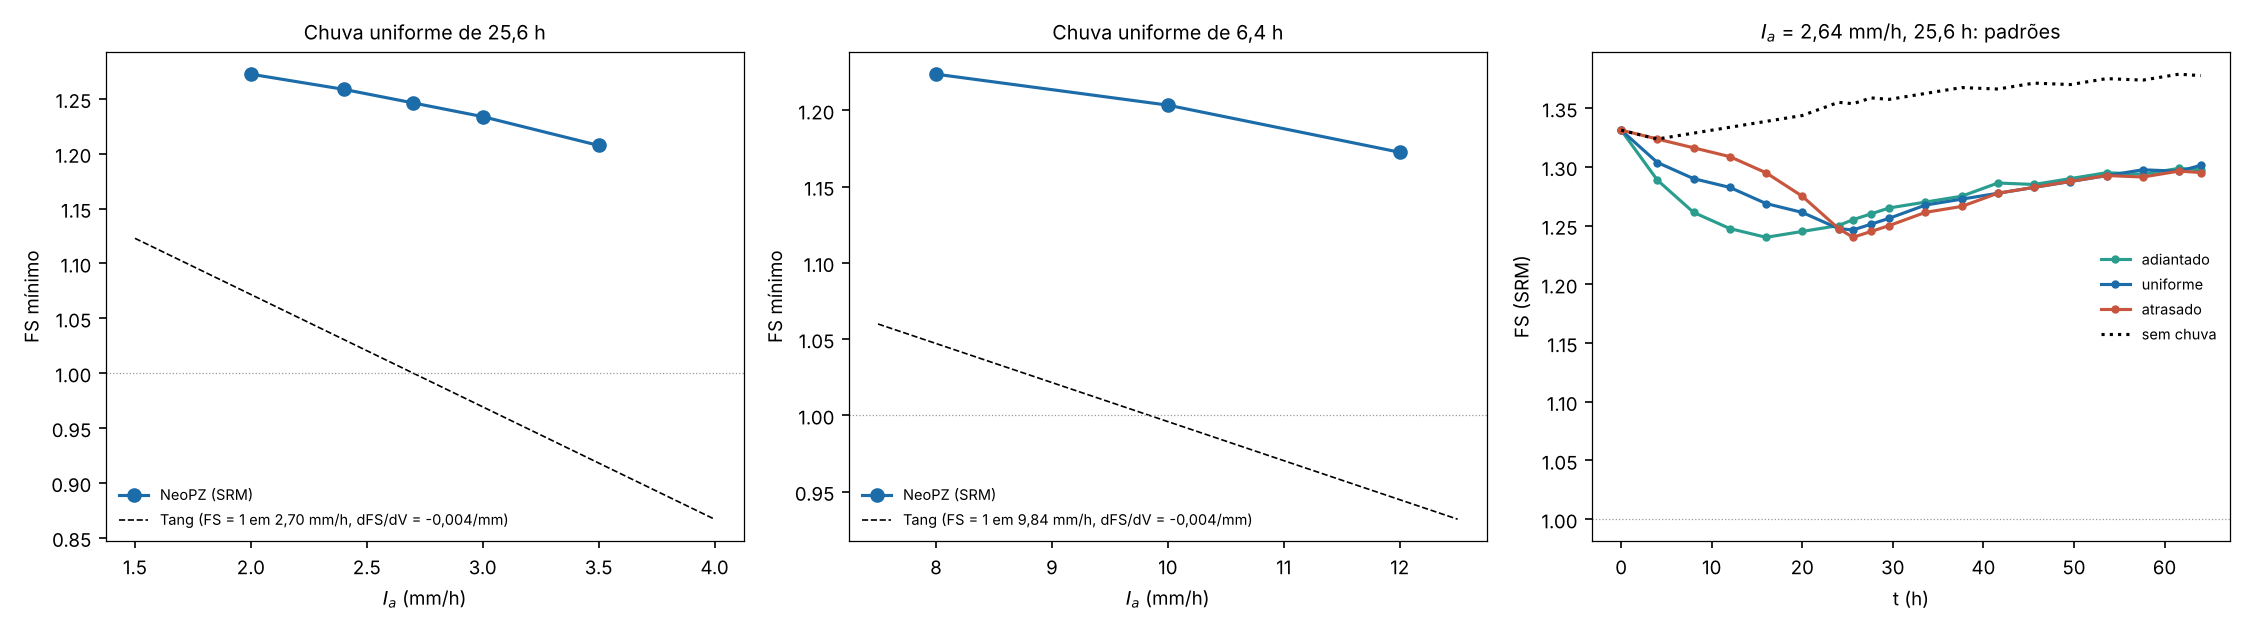
\includegraphics[width=\textwidth]{figuras/tang_fs.png}
\caption{Tang et al.\ (2018) no NeoPZ: FS m\'inimo em fun\c{c}\~ao da intensidade m\'edia nas chuvas de 25,6 e 6,4~h
(tracejado: reta da Fig.~10 do artigo, que passa por FS $=1$ em $I_c$ com a inclina\c{c}\~ao de cada dura\c{c}\~ao) e FS
no tempo para os tr\^es padr\~oes com 2,64~mm/h e sem chuva.}\label{fig:tang}
\end{figure}

As tend\^encias s\~ao as do artigo (o FS cai com o volume; com o mesmo volume, a chuva mais curta reduz mais o FS: com
51 e 77~mm, 0,05--0,06 a menos em 6,4~h do que em 25,6~h; em Tang, FS $=1$ com 62~mm em 6,4~h e 69~mm em 25,6~h), mas
os valores n\~ao: o FS inicial \'e 11\% maior e a queda por mm de chuva, medida contra o c\'alculo sem chuva, \'e
$-0{,}0016$/mm nas chuvas de 25,6~h e $-0{,}0020$/mm nas de 6,4~h, contra $-0{,}0039$ e $-0{,}0047$/mm no artigo
(Fig.~10), de modo que nenhum caso chega a FS $=1$ (1,17--1,27). As verifica\c{c}\~oes a seguir separam as causas:
\begin{itemize}
\item \emph{M\'etodo de estabilidade.} Um Bishop simplificado com busca de c\'irculos (\texttt{scripts/bishop.py})
sobre o mesmo campo inicial d\'a 2,092 no caso de Rahardjo (2,119 no SRM) e 1,298 no de Tang (1,331 no SRM). Os dois
m\'etodos concordam; os 1,20 do artigo n\~ao saem dos par\^ametros publicados.
\item \emph{Campo inicial.} Neste talude o FS de Bishop \'e linear no limite de suc\c{c}\~ao: 0,93, 1,06, 1,18 e 1,30
com 20, 30, 40 e 50~kPa ($\approx0{,}012$ por kPa). O FS inicial do artigo corresponde a um limite de $\approx41$~kPa,
e o FS $=1$ a uma perda m\'edia de $\approx16$~kPa ao longo do c\'irculo cr\'itico; no NeoPZ a perda equivalente \'e
de $\approx7$~kPa.
\item \emph{Percola\c{c}\~ao $\times$ estabilidade.} O Bishop aplicado aos campos de $p_w$ do NeoPZ d\'a a mesma queda
que o SRM ($-0{,}082$ contra $-0{,}085$ ao fim da chuva de 2,7~mm/h): a diferen\c{c}a para o artigo est\'a na
percola\c{c}\~ao, n\~ao no c\'alculo do FS.
\item \emph{Fluxo na face.} No SEEP/W o fluxo prescrito \'e por unidade de comprimento do contorno, o que d\'a
$1/\cos45^\circ=1{,}41$ vez mais \'agua na face do que a chuva na proje\c{c}\~ao horizontal usada aqui. Com essa
conven\c{c}\~ao (op\c{c}\~ao \texttt{fluxonormal=1}) a queda em rela\c{c}\~ao ao FS inicial passa de $-0{,}085$ para
$-0{,}116$: cerca de um quarto da diferen\c{c}a para o artigo (de 1,20 a 1,00).
\item \emph{Padr\~ao da chuva.} Com 2,64~mm/h o padr\~ao muda o instante do FS m\'inimo (16~h no adiantado, 25,6~h
nos outros dois), mas n\~ao o seu valor (1,240 a 1,246, dentro da resolu\c{c}\~ao do SRM). No artigo o atrasado \'e
o mais cr\'itico ($I_c$ de 2,55 contra 2,77~mm/h no adiantado, leitura da Fig.~10) e os padr\~oes aleat\'orios
espalham o FS m\'inimo de 0,86 a 1,05; nos concentrados no fim da chuva o FS continua caindo at\'e 33--39~h, enquanto
no NeoPZ a queda termina com a chuva.
\end{itemize}
H\'a ainda uma raz\~ao f\'isica para a queda pequena: com esses par\^ametros $k_w$ a 50~kPa vale $0{,}54\,k_s\approx
3{,}9$~mm/h, acima das intensidades cr\'iticas do artigo (2,6--2,8~mm/h). Com o limite de 50~kPa essa \'e a
condutividade junto \`a superf\'icie e em toda a zona a mais de 5,1~m acima do NA: o perfil inicial, que n\~ao est\'a em
equil\'ibrio, drena por gravidade (sem chuva o FS cai de 1,33 para 1,32 em 4~h e sobe at\'e 1,38 em 64~h). As chuvas
de 25,6~h (2 a 3,5~mm/h) s\'o reduzem essa drenagem na crista, mas umedecem o p\'e e a face por baixo (ao fim da chuva
a poropress\~ao nos 3~m superiores do p\'e est\'a at\'e 14~kPa (2~mm/h) a 22~kPa (3,5~mm/h) acima da inicial); s\'o as
de 6,4~h (8 a 12~mm/h) criam uma frente de umedecimento a partir da superf\'icie. A sensibilidade
$\mathrm{d}\,\mathrm{FS}/\mathrm{d}V$ do artigo, usada na tese T5, depende portanto do modelo de percola\c{c}\~ao: com
os mesmos dados o NeoPZ d\'a cerca de 40\% dela.

\subsection{Pradhan et al.\ (2022): corte de estrada e encosta natural}

Escorregamento de Kanglang (Nepal), em julho de 2018 (antes de 16/07, segundo o propriet\'ario; 12/07 na
retroan\'alise do artigo), numa encosta de silte de $22^\circ$ com um corte de estrada de 4~m ($71^\circ$) no p\'e
(geometria lida da Fig.~7 do artigo; malhas de $\approx6200$ tri\^angulos, com e sem o corte). Quatro camadas paralelas
\`a superf\'icie natural da encosta (0--0,5, 0,5--1, 1--1,5 e $>1{,}5$~m; a plataforma da estrada e quase toda a face
do corte ficam na camada~4) com as propriedades da Tabela~2: $c'=3$~kPa, $\phi'=36^\circ$, $k_s$ de
$2{,}4\times10^{-7}$ a $5{,}8\times10^{-7}$~m/s (0,9 a 2,1~mm/h), van Genuchten--Mualem (ramo de umedecimento,
$S_{wr}=0$) e $\chi=S_e$ (como no PLAXIS). NA 15~m abaixo da superf\'icie natural (sob a plataforma da estrada, 11,7 a
15~m), laterais imperme\'aveis e base aberta; estado inicial de infiltra\c{c}\~ao permanente com
$3{,}3\times10^{-8}$~m/s (o artigo aplica esse fluxo por cinco anos); chuva hor\'aria de 1 a 12/07/2018 (271~h,
278~mm, seis eventos principais de 27 a 60~mm) digitalizada da Fig.~10 e evapotranspira\c{c}\~ao de 4~mm/dia nos
per\'iodos secos, limitada \`a carga de press\~ao de $-30$~m; percola\c{c}\~ao desacoplada com $p_a=0$; FS por
redu\c{c}\~ao de resist\^encia no estado inicial e em 14 instantes (antes e depois de cada evento). O artigo usa o
modelo acoplado do PLAXIS~2D, tamb\'em com redu\c{c}\~ao de resist\^encia, e simula antes a chuva de dezembro de 2017 a
junho de 2018.

\begin{table}[h!]
\centering\small
\caption{Pradhan et al.\ (2022): FS com o corte e sem o corte, no NeoPZ e no artigo (leitura da Fig.~10).}
\label{tab:pradhan}
\begin{tabular}{rcccc}
\toprule
& \multicolumn{2}{c}{com o corte} & \multicolumn{2}{c}{sem o corte}\\
$t$ (h) & NeoPZ & artigo & NeoPZ & artigo\\
\midrule
0 & 1,956 & 1,79 & 2,734 & 2,75\\
34 & 1,942 & 1,75 & 2,733 & 2,72\\
42 & 1,767 & 1,46 & 2,713 & \\
96 & 1,904 & 1,71 & 2,724 & 2,71\\
101 & 1,676 & 1,42 & 2,704 & \\
167 & 1,888 & 1,82 & 2,716 & 2,72\\
173 & 1,606 & 1,46 & 2,688 & \\
184 & 1,680 & 1,62 & 2,699 & \\
200 & 1,365 & 1,12 & 2,664 & \\
216 & 1,512 & 1,42 & 2,669 & 2,68\\
222 & 1,293 & 1,13 & 2,649 & \\
261 & 1,468 & 1,29 & 2,636 & 2,65\\
264 & 1,314 & 1,10 & 2,622 & \\
267 & 1,170 & 0,97 & 2,608 & \\
271 & 1,150 & 1,00 & 2,601 & 2,62\\
\bottomrule
\end{tabular}
\end{table}

\begin{figure}[h!]
\centering
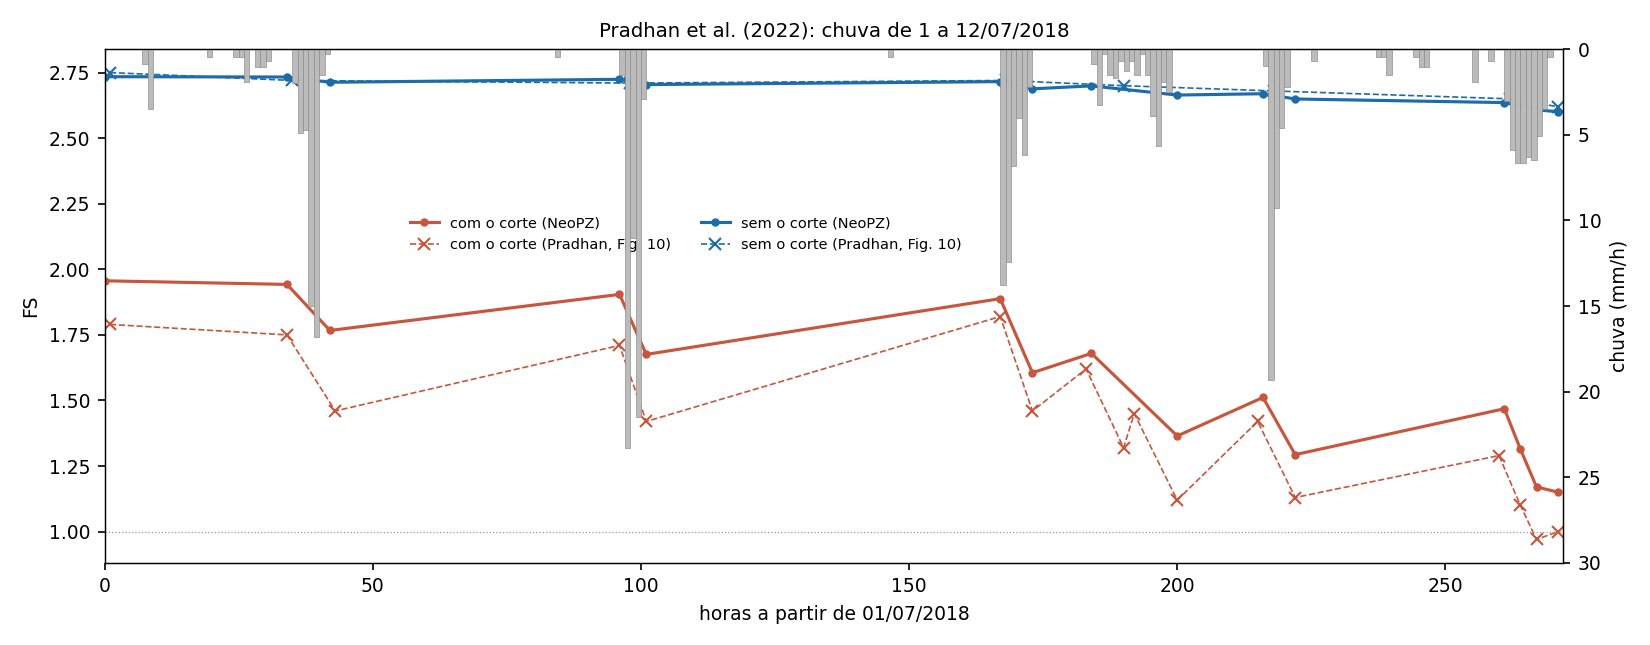
\includegraphics[width=\textwidth]{figuras/pradhan_fs.png}
\caption{Pradhan et al.\ (2022): FS durante a chuva de 1 a 12/07/2018 com o corte e sem o corte, no NeoPZ e no
artigo (leitura da Fig.~10); barras: chuva hor\'aria digitalizada.}\label{fig:pradhan}
\end{figure}

Com o corte, o NeoPZ reproduz a forma da resposta: o FS cai em cada um dos seis eventos, recupera em parte nos
intervalos secos (drenagem e evapotranspira\c{c}\~ao) e tem o m\'inimo no fim (1,15 em 271~h; o artigo prev\^e a
ruptura em 267~h, com 0,97). O n\'ivel fica 4 a 22\% acima do artigo (FS inicial 1,96 contra 1,79) e as quedas por
evento s\~ao menores (0,18 a 0,31, com o evento 6 at\'e 267~h, contra 0,29 a 0,50 no artigo, isto \'e, 61 a 93\%), o
mesmo padr\~ao encontrado em Tang. A maior queda nos dois modelos \'e a do evento 4, o de menor volume de chuva (27~mm)
e maior dura\c{c}\~ao (15~h): nele infiltram 79\% da chuva, contra 32 a 53\% nos outros cinco eventos, mais curtos e
intensos. O volume infiltrado sozinho, por\'em, n\~ao ordena as quedas: o evento 3 infiltra mais (24,1 contra 21,7~mm)
e cai menos (0,28), e a queda por mm infiltrado passa de 0,010 no evento 1 a 0,021 no evento 6; o artigo l\^e o efeito
como da dura\c{c}\~ao (Fig.~13).

Sem o corte a encosta quase n\~ao reage \`a chuva: o FS cai devagar de 2,73 para 2,60 em 271~h, a menos de 0,04 da
leitura da Fig.~10 (2,75 para 2,62). O FS inicial \'e 40\% maior sem o corte (54\% no artigo) e, no fim da chuva,
$\approx130\%$ maior ($\approx160\%$ no artigo): a conclus\~ao do artigo, de que o corte \'e o que torna a chuva de
julho cr\'itica, se mant\'em.

Tr\^es diferen\c{c}as de modelo podem explicar o n\'ivel mais alto com o corte: (i) o estado inicial, que aqui \'e a
infiltra\c{c}\~ao permanente e no artigo \'e o fim da simula\c{c}\~ao de dezembro a junho (com FS $<1$ em junho, mais
\'umido em 1$^\circ$ de julho); (ii) a regra de escoamento: o PLAXIS usa $\psi=0$ por padr\~ao e o artigo, num silte
contr\'atil, n\~ao informa $\psi$, enquanto a redu\c{c}\~ao de resist\^encia do NeoPZ \'e sempre associativa (o
execut\'avel n\~ao associativo d\'a o mesmo FS inicial, 1,956, com $\psi=0$, porque tamb\'em calcula o FS com
$\psi=\phi$); com $\phi'=36^\circ$ essa diferen\c{c}a pode ser relevante, mas n\~ao foi testada; (iii) a resposta da
percola\c{c}\~ao a cada evento, menor aqui como no caso de Tang (nas quedas por evento pesam tamb\'em o acoplamento,
ausente aqui, e a leitura da chuva numa figura). O caso sem o corte, pouco sens\'ivel a essas diferen\c{c}as, mostra
que a geometria, as camadas, o NA e a chuva digitalizada est\~ao corretos.

%======================================================================
\section{O patamar inferior do FS}\label{sec:patamar}
%======================================================================

Com $I_r$ acima da capacidade de infiltra\c{c}\~ao a superf\'icie alaga ($p_w=0$) e o solo abaixo dela satura
progressivamente. O FS decresce at\'e o estado do talude saturado at\'e a superf\'icie, com a \'agua escoando por ele;
esse estado depende da geometria, da resist\^encia, das condi\c{c}\~oes de contorno hidr\'aulicas e da forma do tensor de
condutividades (anisotropia), mas n\~ao da magnitude de $k_s$ nem da intensidade, que s\'o determinam quando ele \'e
atingido. O c\'alculo direto usa a op\c{c}\~ao \texttt{alagado=1} ($p_w=0$ em toda a superf\'icie, $I\to\infty$) com o
modelo do artigo (percola\c{c}\~ao desacoplada, $p_a=0$) e \texttt{mecanica=0} (o transiente resolve s\'o a
percola\c{c}\~ao e o SRM parte do estado sem tens\~oes com as press\~oes congeladas; Tabela~\ref{tab:patamar}).

\begin{table}[h!]
\centering\footnotesize\setlength{\tabcolsep}{4pt}
\caption{FS (SRM) com a superf\'icie alagada desde $t=0$ (em negrito, a primeira sa\'ida j\'a no patamar), faixa do FS
desse instante at\'e o tempo final $t_f$ e patamar das chuvas intensas (s\'erie B desacoplada e item A3). Anisotropia:
$k_1=10^{-4}$, $k_2=10^{-5}$~m/s. $^\dagger$FS m\'inimo das chuvas de 24~h, que no $f_{100}$ n\~ao atingem o patamar
(Eq.~6: 1,45).}\label{tab:patamar}
\begin{tabular}{lccccccccc}
\toprule
caso & 1~h & 3~h & 6~h & 12~h & 24~h & 96~h & 192~h & at\'e $t_f$ & com chuva\\
\midrule
$f_{10}$ isotr\'opico & 1,44 & 1,15 & 0,98 & \textbf{0,85} & 0,84 & 0,84 & 0,85 & 0,84--0,85 (384~h) & 0,84\\
$f_{50}$ isotr\'opico & & 1,58 & 1,36 & 1,17 & \textbf{0,85} & 0,84 & 0,85 & 0,84--0,85 (1536~h) & 0,84--0,85\\
$f_{100}$ isotr\'opico & & & 1,88 & & 1,49 & 1,06 & \textbf{0,85} & 0,84--0,85 (6144~h) & 1,48$^\dagger$\\
$f_{50}$, $\theta=0^\circ$ & & 1,30 & 1,21 & 1,13 & \textbf{1,05} & 1,04 & 1,05 & 1,04--1,05 (768~h) & 1,05\\
$f_{50}$, $\theta=45^\circ$ & & 1,00 & \textbf{0,88} & 0,87 & 0,87 & 0,88 & 0,88 & 0,87--0,88 (768~h) & 0,87\\
$f_{50}$, $\theta=135^\circ$ & & 1,27 & \textbf{0,63} & 0,63 & 0,63 & 0,63 & 0,63 & 0,63 (768~h) & 0,63\\
\bottomrule
\end{tabular}
\end{table}

\begin{figure}[h!]
\centering
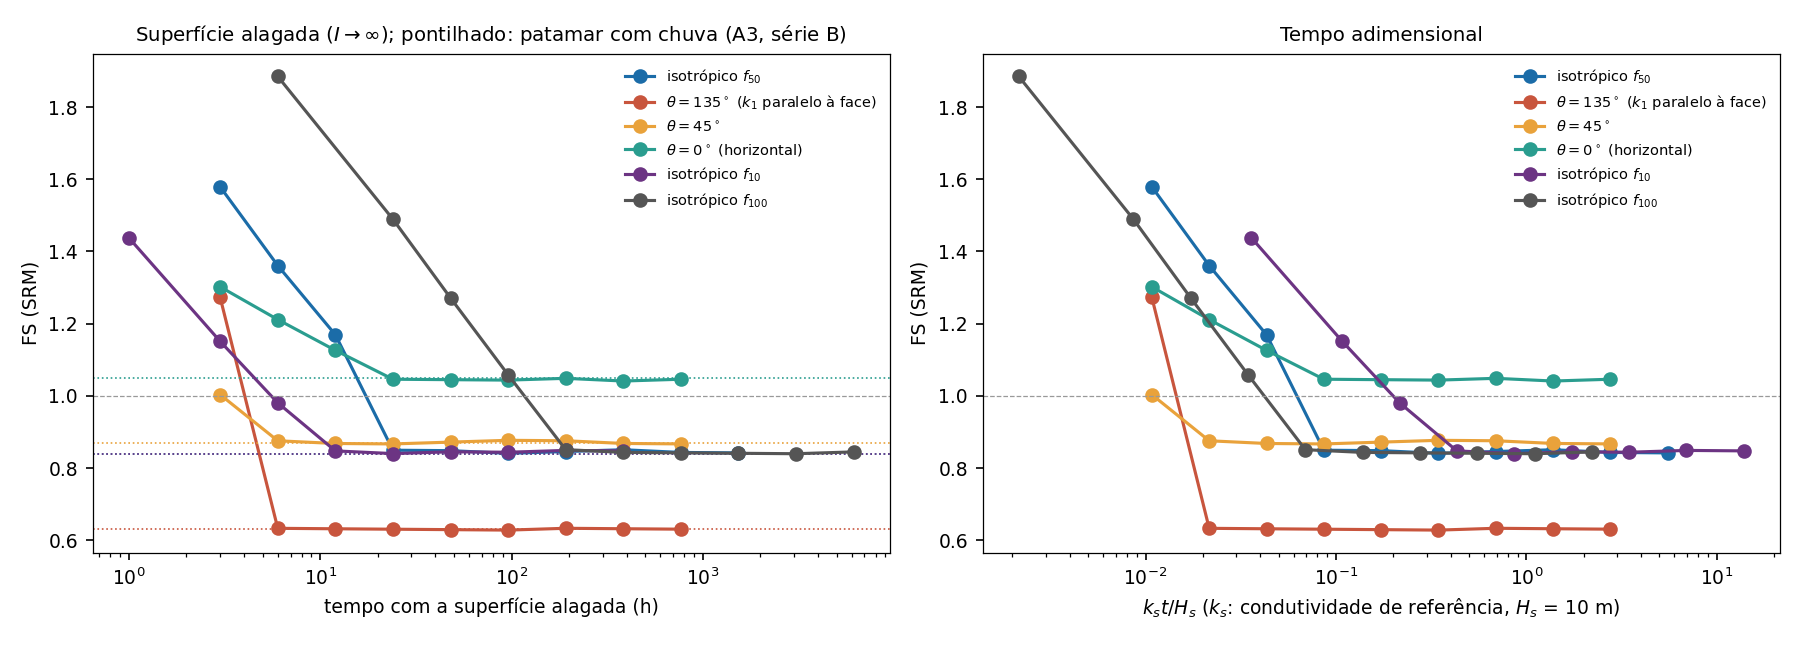
\includegraphics[width=\textwidth]{figuras/patamar_alagado.png}
\caption{FS com a superf\'icie alagada desde $t=0$ (modelo do artigo: percola\c{c}\~ao desacoplada, $p_a=0$), em tempo
real e em tempo adimensional $k_st/H_s$. Pontilhado: patamar das chuvas intensas (s\'erie B desacoplada e item A3).}
\label{fig:patamar}
\end{figure}

\begin{itemize}
\item O patamar \'e o mesmo nos tr\^es solos (0,84--0,85) e \'e um regime permanente: o $f_{10}$ o atinge em
$\approx7$~h, o $f_{50}$ em $\approx24$~h e o $f_{100}$ em $\approx170$~h (in\'icio da infiltra\c{c}\~ao constante; nas
sa\'idas do FS, entre 6 e 12~h, 12 e 24~h e 96 e 192~h), e da\'i at\'e o fim do c\'alculo (384, 1536 e 6144~h) o FS
n\~ao sai da faixa 0,84--0,85 (Fig.~\ref{fig:patamar}). O valor 1,45 do $f_{100}$ na Eq.~6 \'e o FS ao fim de 24~h de
chuva, n\~ao um patamar: a ``intensidade-limite'' do artigo \'e, para o solo pouco perme\'avel, um efeito da
dura\c{c}\~ao fixa.
\item O FS com a superf\'icie alagada reproduz o patamar das chuvas intensas nos cinco casos em que a chuva de 24~h o
atinge ($f_{10}$, $f_{50}$ e os tr\^es anisotr\'opicos, 0,63 a 1,05) e, no $f_{100}$, o FS ao fim das 24~h (1,49 contra
1,48--1,50): a orienta\c{c}\~ao do tensor muda a rede de fluxo do talude saturado e, com ela, o patamar.
\item Consequ\^encia pr\'atica: o patamar inferior \'e calcul\'avel sem simular a chuva, com um \'unico c\'alculo com a
superf\'icie alagada at\'e o regime permanente. O tempo para atingi-lo cresce com $1/k_s$, mas n\~ao na mesma
propor\c{c}\~ao: do $f_{50}$ para o $f_{100}$ ele aumenta $\approx7$ vezes e do $f_{10}$ para o $f_{50}$ $\approx3$ (em
tempo adimensional $k_st/H_s$, $\approx0{,}26$ no $f_{10}$, $\approx0{,}09$ no $f_{50}$ e $\approx0{,}06$ no $f_{100}$),
porque o volume a infiltrar at\'e o regime permanente depende da curva de reten\c{c}\~ao (o $f_{10}$ parte da menor
satura\c{c}\~ao). Compare com a dura\c{c}\~ao cr\'itica de um volume fixo, Eq.~\eqref{eq:tcrit}.
\end{itemize}

Nos c\'alculos com a superf\'icie alagada por muito tempo o Newton da percola\c{c}\~ao deixava de convergir depois de
atingido o regime permanente: o res\'iduo j\'a estava no n\'ivel do arredondamento e a busca linear, sem conseguir
reduzi-lo, marcava o passo como n\~ao convergido. A busca linear agora s\'o \'e feita enquanto a corre\c{c}\~ao de
press\~ao excede a toler\^ancia (o mesmo defeito interrompeu os casos de 360~mm/h do item A3 e de 360 e 900~mm/h do
$f_{10}$ na S\'erie B). Com a corre\c{c}\~ao, os seis casos da Tabela~\ref{tab:patamar} chegaram ao tempo final, e o
FS ficou na faixa de $\pm0{,}005$ do patamar por 30 a 130 vezes o tempo em que ele foi atingido; os cinco casos
interrompidos, refeitos, ca\'iram no patamar: 0,84 no $f_{10}$ com 360 e 900~mm/h e 1,05, 0,87 e 0,63 nos
anisotr\'opicos com 360~mm/h (Tabelas~\ref{tab:B} e \ref{tab:A3}).
